\subsection{The Diffraction Grating}

A diffraction grating is a plate with \textbf{many closely spaced parallel slits} ruled on it. When a beam of \textbf{monochromatic light} is directed a diffraction grating, light is transmitted in \underline{certain directions only}.
\begin{itemize}
    \item The light passing through each slit is \textbf{diffracted}.
    \item The diffracted waves from adjacent slits reinforce each other in \textbf{certain directions only}.
\end{itemize}

The \textbf{zero order beam} is in the same direction as the incident beam.

The \textbf{angle of diffraction} between each transmitted beam and the central beam increases if
\begin{itemize}
    \item Light with a \textbf{longer wavelength} is used.
    \item Grating with \textbf{closer slits} is used.
\end{itemize}

Each diffracted wavefront emerges from a slit and \textbf{reinforces a wavefront} from a slit adjacent to it.
\begin{center}
    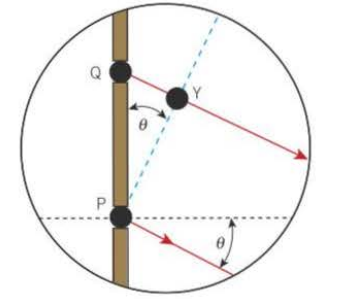
\includegraphics[width=4cm]{img/grating}
\end{center}
\begin{itemize}
    \item The distance $QY$ from the slit to the wavefront is equal to $n\lambda$.
    \item The \textbf{angle of diffraction} of the beam $\theta$ is equal to the angle between the wavefront and the plate of the slits.
    \item So $\sin\theta=n\lambda/d$ where $d$ is the \textbf{grating spacing}.
\end{itemize}
$$d\sin\theta=n\lambda$$
for the $n$th order beam.

The \textbf{maximum number of orders} is given by the value $d/\lambda$ rounded down to the nearest whole number.

\subsubsection*{Types of Spectra}

\begin{itemize}
    \item \textbf{Continuous spectra} - the hotter the light source, the shorter the wavelength of the brightest part of the spectrum.
    \item \textbf{Line emission spectra} - consists of \textbf{narrow vertical lines} of different colour. The wavelengths of the lines are \textbf{characteristic of the chemical element} that produced the light.
    \item \textbf{Line absorptions spectra} - a continuous spectrum with \textbf{narrow dark lines} at certain wavelengths. Atoms of glowing gas absorb light then emit light subsequently, but not necessarily in the same direction as the transmitted light.
\end{itemize}
